\section{Classical simulation}
\label{sec:classical}
While the currently applied traditional methods for the analysis of experimental scattering data discussed previously are popular.
There is growing interest in the use of multi-modal analysis methods that leverage classical simulation to assist in the analysis of scattering data.\autocite{ivanovic_temperature-dependent_2018,scoppola_combining_2018,dabkowska_modulation_2014,hub_interpreting_2018}
This would involve the simulation of the chemical system in order to educate the analysis of the experimental data.
These systems, especially when the materials being simulated are soft in nature, are often highly complex and typically cover large length scales.
Classical simulation, particularly in combination with coarse-grained potential models, can feasibly enable the simulation of these systems.

In order to simulate the complexity of a real chemical system, it is necessary to model the electrons of the molecules and their interactions.
This is usually achieved using quantum mechanical calculations, where the energy of the system is calculated by finding some approximate solution to the Schr\"{o}dinger equation.
However, quantum mechanical calculations are very computationally expensive and are realistically limited to hundreds of atoms.
In order to simulate a soft matter system such as a phospholipid monolayer or polymer nanoparticles, it is necessary to simplify the calculation being performed.
This leads to the use of classical simulations, where parameterised analytical functions are used to represent the potential energy of the system.
Classical simulations are used substantially in this work, in terms of molecular dynamics simulations.\footnote{Molecular dynamics (MD) is discussed in detail in Section~\ref{sec:optimisation}.}
Therefore, it is necessary to introduce the underlying theory on which this method is defined.

\subsection{Potential models}
\label{sec:potentmodels}
Potential modelling is a more computationally efficient method for the calculation of the potential energy of a chemical system.
A potential model consists of a series of mathematical functions that depend on the atomic positions, $\mathbf{r}$.
Each of the functions represents the potential energy of a different interaction for a given atom.
Broadly, these interactions can be split into bonded and non-bonded, such that the total energy may be described as follows,
%
\begin{equation}
\begin{aligned}
  E_{\text{total}}(r) = & \sum_{\text{bonded pairs}}{E_{\text{bonded}}(r)} \\
  & + \sum_{\text{atom pairs}}{E_{\text{non-bonded}}(r)}.
\end{aligned}
\end{equation}
%
The total potential energy is then the sum of the potential energy for each of the individual atoms.

The bonded terms are used to describe different aspects of chemical bonds.
These typically consist of bond stretches, angle bends and dihedral torsions, these interactions have the following mathematical form,\footnote{These forms are specific to the OPLS2005 potential model (\cite{banks_integrated_2005}), other potential models may have different functions.}
%
\begin{equation}
\begin{aligned}
  E_{\text{bonded}}(b, \theta, \phi) = & \sum_{\text{bonds}}K_b(b-b_0)^2 + \sum_{\text{angles}}K_{\theta}(\theta-\theta_0)^2 \\
  & + \sum_{\text{dihedrals}} \frac{1}{2}\big\{A_1[1 + \cos(\phi)] \\
  & + A_2[1 - \cos(2\phi)] + A_3[1 + \cos(3\phi)]\big\},
\end{aligned}
\end{equation}
%
where, $K_b$ and $b_0$, $K_{\theta}$, $\theta_0$, and $A_1$, $A_2$, and $A_3$ are interaction dependent parameters for the bonds, angles, and dihedrals respectively, while $b$, $\theta$, and $\phi$ are the bond lengths, the size of the angles, and the size of the dihedrals that depend on the atom positions.\footnote{The values for the interaction dependent parametes are determined as outlined in Section~\protect\ref{sec:parameterisation}.}
It can be seen that both the bond stretch and angle bend have harmonic functions, whereas the dihedral consists of a more complex multiple cosine functions.

The non-bonded terms are a series of functions that describe the potential energy of intermolecular interactions, such as electrostatics and London dispersion forces.
The potential energies of the short-range interactions are usually modelled as a combination of the attractive London dispersion interaction and the repulsive exchange forces that arise from the Pauli exclusions principle.\autocite{leach_molecular_1996}
These are often forms such as shown below for the Lennard-Jones potential model,\autocite{lennard-jones_determination_1924}
%
\begin{equation}
\begin{aligned}
  E_{\text{non-boned}}(r) = & E_{\text{repulsive}} + E_{\text{attractive}} \\
  = & \frac{A}{r^{12}} - \frac{B}{r^6} = 4\varepsilon\Bigg[\bigg(\frac{\sigma}{r}\bigg)^{12} - \bigg(\frac{\sigma}{r}\bigg)^6\Bigg]
\end{aligned}
\end{equation}
%
where, $r$ is the distance between two particles, $A$ and $B$ are interaction dependent parameters, and $\sigma$ and $\epsilon$ are simple reformations of these parameters,
%
\begin{equation}
  A = 4\varepsilon\sigma^{12} \;\;\;\; B = 4\varepsilon\sigma^6.
\end{equation}
%
Figure~\ref{fig:lj} shows each component of the Lennard-Jones potential model for atoms of argon.\footnote{Using parameters for $A$ and $B$ determined in \cite{rahman_correlations_1964}.}
The Lennard-Jones potential model is not the only form that may be used for the modelling of the short-range non-bonded interactions, others such as the Buckingham and Morse potentials exist.\autocite{buckingham_classical_1938, morse_diatomic_1929}
In each case, there is a short ranged repulsive interaction to describe the electrostatic repulsion between the electron clouds, and a longer range attractive component that represents dispersion interactions.
However, the Lennard-Jones model has been used heavily in this work.
%
\begin{figure}[t]
    \forceversofloat
    \centering
    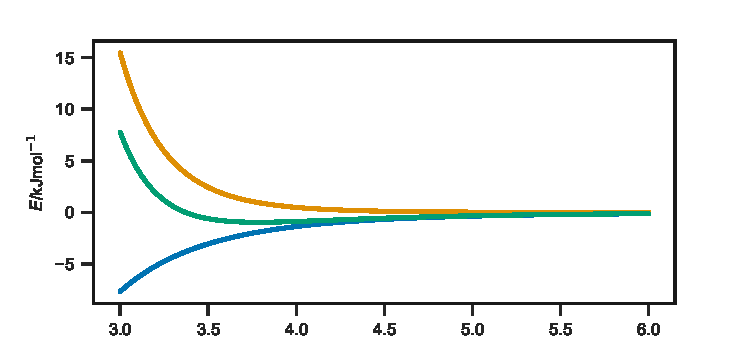
\includegraphics[width=\textwidth]{theory/lj}
    \caption{The form of each component; attractive (blue), repulsive (orange), of the Lennard-Jones potential model (green) for argon, using parameters in \cite{rahman_correlations_1964}.}
    \label{fig:lj}
\end{figure}
%

While the short-range interactions can be accounted for by a function such as the Lennard-Jones potential model, the potential energy of the long-range electrostatic interactions are usually modelled, more consistently, using Coulomb's law for classical electrostatic interaction between point particles,\autocite{coulomb_premier_1788, coulomb_second_1788}
%
\begin{equation}
  E_{\text{Coulomb}}(r) = \frac{1}{4\pi\varepsilon_0}{\frac{q_iq_je^2}{r^2}},
  \label{equ:col}
\end{equation}
%
where, $r$ is the distance between the two particles, $\varepsilon_0$ is the dielectric permittivity of the vacuum, $e$ is the charge of the electron, and $q_i$ and $q_j$ are the electronic charges on each of the particles.
It is clear that when $q_i$ and $q_j$ have the opposite signs Coulomb's law is always attractive.
The fact that Equation~\ref{equ:col} contains a factor of $r^2$ indicates that this is a much longer range interaction than those modelled with the Lennard-Jones model, make the Coulomb potential more complex to compute.\autocite{frenkel_understanding_1996}

An example of a very large classical simulation would be $\sim3$ million atoms.\autocite{gumbart_regulation_2009}
However, this is still only \SI{1.8e-16}{\mol} which is not remotely realistic as a simulation of a ``real'' system.
A common method to allow for the apparent simulation of a much larger system is the use of periodic boundary conditions.\footnote{Abbreviated to PBC.}
This is where a boundary condition is applied to the edges of the simulation cell, such as to mimic an infinite system, such that the simulation cell is surrounded by identical images of itself, this is shown pictorially in Figure~\ref{fig:pbc}.
Using the PBC means that atomic diffusion is conserved as when an atom reaches the edge of the simulation cell, it will appear on the other side as though it came from the adjacent periodic cell.
The use of a PBC is particularly powerful in the simulation of homogenous systems, such as liquids.
%
\begin{figure}[b]
    \forceversofloat
    \centering
    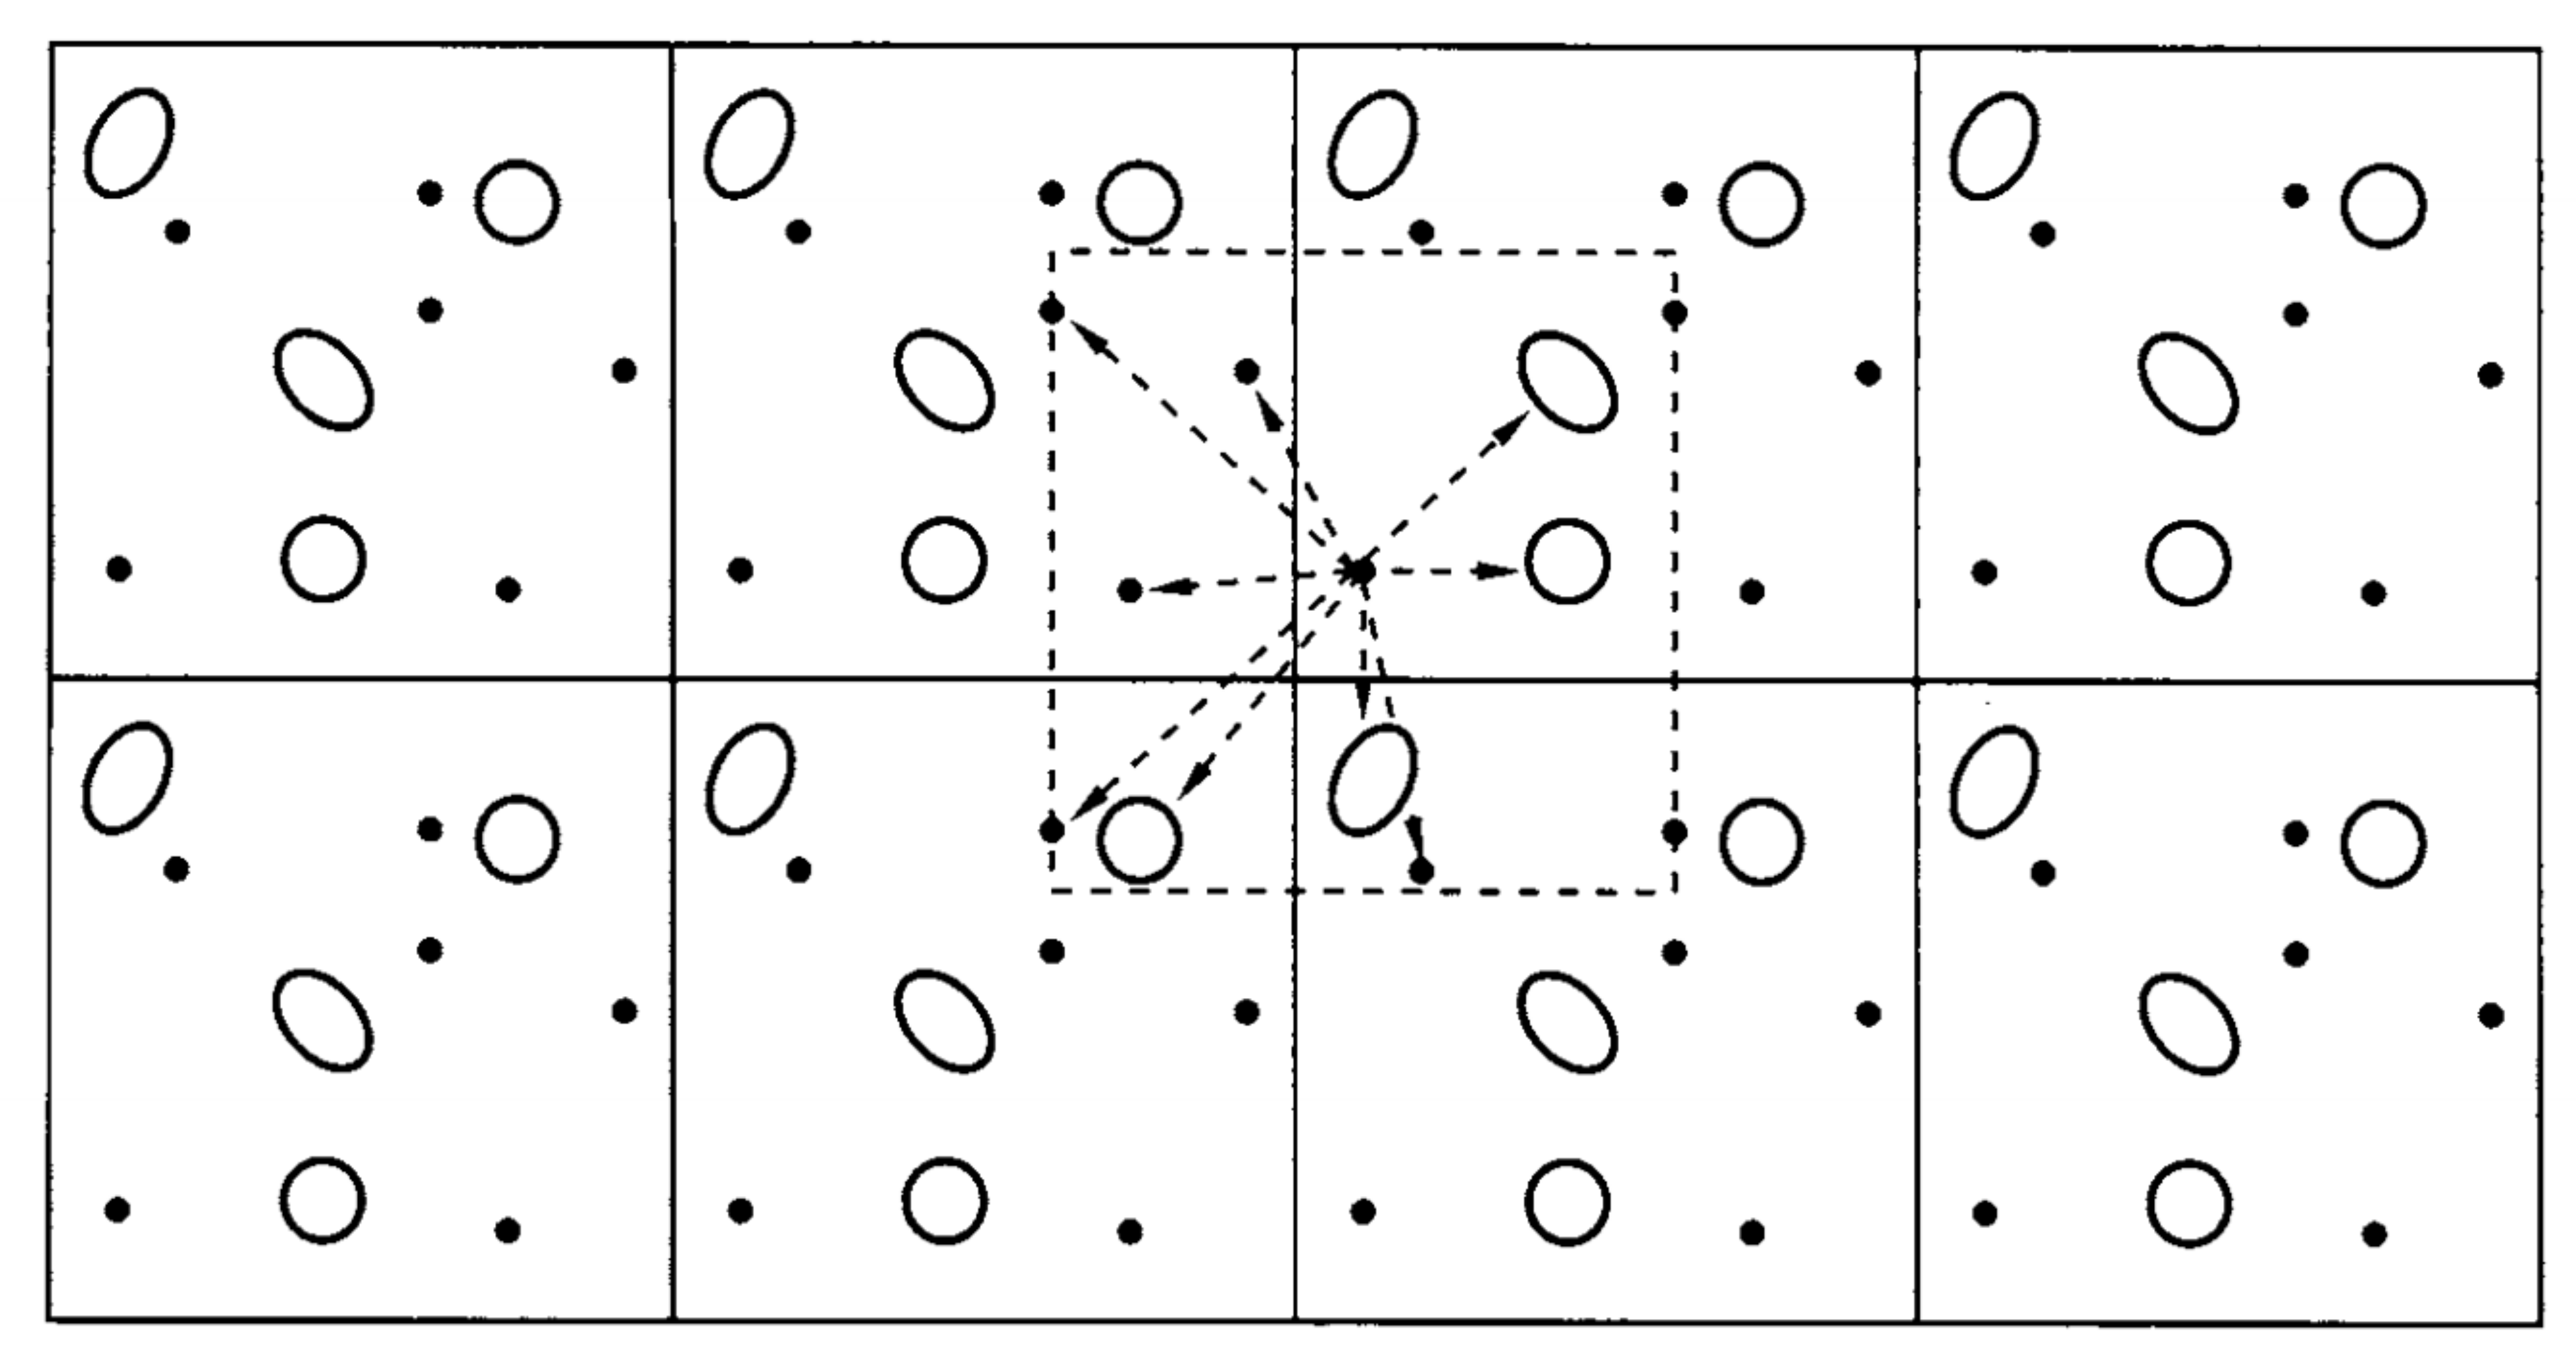
\includegraphics[width=0.8\textwidth]{theory/pbc}
    \caption{A graphical representation of the PBCs. Reprinted, with permission of Elsevier, from \cite{frenkel_understanding_1996}.}
    \label{fig:pbc}
\end{figure}
%

The cut-off is another important factor for classical simulation, this is the distance after which the energy between two particles is considered to be zero.
Therefore, for distances greater than the cut-off, it is not necessary to calculate the energy between the two particles as it is taken to be zero.\footnote{This leads to an increase in computational efficiency.}
Code Block~\ref{cb:lj} gives an example of some code that could be used to calculate the Lennard-Jones energy of an atomistic system, where both the PBC and the energy cut-off distance are considered.
%
\begin{listing}[b]
    \forcerectofloat
    \centering
    \caption{Code that may be used to generate the Lennard-Jones energy for a given atomistic system, which accounts for the PBC and the energy cut-off distance. The input varibles are \texttt{coordinates} which is an array of floats describing the position of the \texttt{N} particles, \texttt{cell} which are the unit cell vectors, \texttt{cut\_off} which is potential energy cut-off, and \texttt{A} and \texttt{B} which are the Lennard-Jones potential parameters. This returns an array with the energy for each particle.}
    \lstinputlisting[nolol]{reports/code_blocks/lennardjones.py}
    \label{cb:lj}
\end{listing}
%

The use of the PBC may be problematic for systems containing long-range interactions, such as classical electrostatics, due to the fact that the range of the electrostatic interaction may be much greater than the size of half of the simulation cell, which can be taken to be the energy cut-off distance.
In order to avoid truncation artefacts, the Ewald summation is often used for the calculation of the electrostatic contribution to the potential energy.\autocite{ewald_berechnung_1921}
The Ewald summation involves performing the summation of the contributing interaction energies in reciprocal space rather than in real space as is the case for the short-range interactions.
Most modern MD simulation software packages implement the Ewald summation using a particle mesh Ewald method.\autocite{essmann_smooth_1995}

\subsection{Parameterisation}
\label{sec:parameterisation}
Section~\ref{sec:potentmodels} introduced the idea of potential models that may be used to evaluate the potential energy of a given system, requiring much less time than methods that rely on the use of quantum mechanics.
However, for these methods to be effective, it is important that the potential models used are able to model the system under study accurately.
This is achieved initially by selecting the correct potential model for a given interaction, and then by ensuring that the interaction-dependent parameters are accurate for a given interaction.
The method of obtaining such parameters is referred to as ``parameterising'' the model.
Model parameterisation is important for all types of potential models, for example it is necessary to determine the equilibrium bond length $b_0$ and the force constant $K_b$ for a given covalent bonds, or the partial electrostatic charge that is present on a carbonyl oxygen atom when it interacts with the hydrogen atom from a neighbouring hydroxyl group.

Parameterisation of a potential model is usually achieved by fitting the potential model functions to energetic data obtained using a higher accuracy technique.\footnote{These may be quantum mechanical calculations or experimental methods.}
We will not dwell on the details of potential model parameterisation,\footnote{This is discussed in detail in many textbooks such as \cite{harvey_computational_2018,leach_molecular_19962}} however, it is important to note that the parameters used in MD simulation are not absolute and depend heavily on the merits of the parameterisation method.

In this work, we have focused heavily on the use of off-the-shelf potential models, to ensure the easy replicability of the work.
Off-the-shelf potential models are those that are determined to be applied to a wide range of chemical systems.
An example includes the OPLS potential model which was parameterised by comparison to quantum mechanical measurements and crystallographic data.\autocite{jorgensen_opls_1988}
While these off-the-shelf potential models are useful for their ease-of-use, it is noted that often these forcefields may require optimisation for the particular system.

\subsection{Coarse-graining}
\label{sec:coarsegraining}
The atomistic simulation of very large systems, such as multiple surfactant micelles or large phospholipid monolayers, require a huge number of atoms.
While computational efficiency improvements such as the PBC or the energy cut-off distance are able to reduce the time taken to simulate these systems, it is often still not possible to produce physically meaningful simulations,\footnote{In particular for emergent properties that depend on large system sizes and long simulation times.} without including some other efficiency improvements.

This has led to the use of coarse-graining of molecules in simulations.
This is the definition of super-atoms, in the place of groups of atoms, known as ``beading'', some examples are shown for the MARTINI force field\autocite{marrink_martini_2007} in Figure~\ref{fig:cg}.
Each of the super-atoms must correspond to the chemistry of the underlying atoms.
For example, the MARTINI potential model introduces five different apolar, beads to represent the polarity of the carbon atoms that make up the super-atom.
Additionally, there are thirteen other super-atom types that can be used to model polar, nonpolar, and charged atomic groups.
%
\begin{figure}[t]
    \forcerectofloat
    \centering
    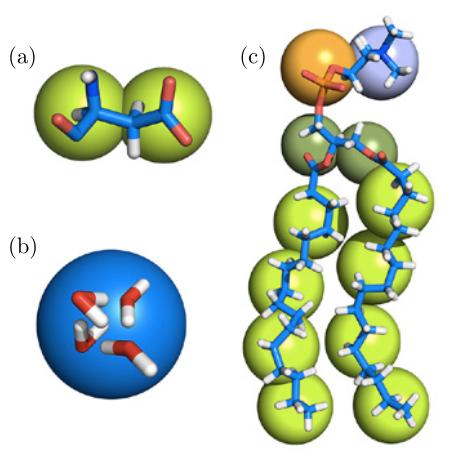
\includegraphics[width=0.8\textwidth]{theory/beading}
    \caption{Three examples of the MARTINI coarse-graining mechanism for (a) aspertic acid, (b) a water cluster, and (c) a molecule of DPPC. Reprinted with permission of the Institute of Physics, from \cite{pluhackova_biomembranes_2015}.}
    \label{fig:cg}
\end{figure}
%

In addition to the computational benefit of having fewer particles in the simulation,\footnote{Therefore requiring fewer integrations of the equations of motion} there is also the opportunity to increase the timestep length for the simulation.\autocite{pluhackova_biomembranes_2015}
This can be achieved as the highest frequency vibrations that must be modelled in the system are integrated out.
For example, another coarse-grained model called the united atom potential model, where the hydrogen atoms have been integrated out, the timestep may be larger than for the same all-atom system as it is no longer necessary to model the high-frequency \ce{C-H} bond.

The technique of coarse-graining a molecule can range from the integration of the hydrogen atoms into the heavier atoms to which they are bound, all the way to the treatment of entire molecules as a single ``bead'', with the inclusion of an implicit solvent.
The parameterisation of a coarse-grained potential model is carried out in much the same way as discussed in Section~\ref{sec:parameterisation} for all-atom potential models.
The coarse-grained parameters are determined by comparison with a higher-resolution technique.\footnote{Often this is all-atom MD simulations.}
